\chapter{硬件架构}

\section{节点}

\subsection{添加节点}

负载均衡,需要重新平衡数据

\subsection{删除节点}

恢复


\section{Pool}

\section{Disk}

画出Disk的状态机

\subsection{Tool}

操作磁盘的工具
\begin{enumbox}
\item hdparm set/get hard disk parameters
\item lsscsi
\item udevadm
\item sg\_inq
\item disk2lid (自己实现的)
\item iostat
\end{enumbox}

\subsection{RAID}

Ctrl+R进入bios的RAID控制界面。通过bios进行的管理操作,进入系统后用MegaCli等命令行工具也能完成。
且更为方便。

每个控制器管理一个或多个enclosure,每个enclosure有固定数量的slot。每个slot对应一块物理设备。
每个物理设备处在不同的firm 状态,这些状态可以相互转换。在物理设备之上,构建虚拟设备。

带电池BBU的情况下,可以打开RAID cache。

NVMe在不在RAID里,系统盘呢?看不到系统盘,是因为系统盘不在RAID控制器管理的slot内?

缓存盘做出JBOD,数据盘RAID0

全部是JBOD,性能影响较大。

\subsection{Cache}

Disk Cache

关闭磁盘cache,防止出现数据不一致情况。怎么关闭呢?相关管理工具是什么?

磁盘的设备驱动,linux kernel的块设备IO架构

NVMe具有什么特征?

\subsection{Meta}

/proc/partitions包含所有分区,过滤掉特定的分区,就是lich可用的设备。
注册到lich的设备定义有自身的元数据:\hl{数据盘包括磁盘头的元数据以及元数据文件}。

数据盘对应的cache设备记录在bcache本身的元数据里,通过sys fs,以及用户态工具管理。

diskid的唯一性在\hl{所有场景}中能否得到保证?

磁盘管理元数据目录:/opt/fusionstack/data/disk:
\begin{compactitem}
\item disk (磁盘在线离线的开关)
\item block (super block)
\item info (diskinfo)
\item \hl{bitmap} (不可丢)
\item tier
\item speed
\end{compactitem}

对每块磁盘,开头的1M是引导信息,通过bitmap来进行空间管理。
引导信息包含了所在节点信息,所以只能在节点内进行磁盘漫游。

\begin{figure}[h]
    \centering
    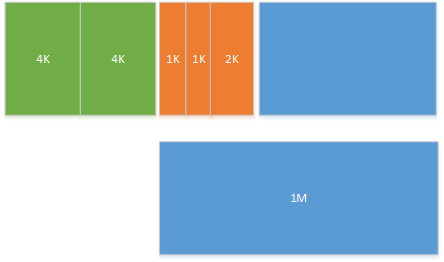
\includegraphics{../images/disk_layout.png}
    \caption{磁盘数据布局}
\end{figure}

磁盘头的元数据布局:MBR(0)+SB(1024)+DISKINFO(4096)。
其中SB包含定义的扩展属性:(cluster, node, type, disk, pool, cache, cached, cset)

每块盘的disk id属性,可用来重建disk/disk目录下的软链接。
block与info文件都可以通过读取磁盘头重建出来。bitmap文件则不可丢。

所在源文件是\emph{diskmd.c}。调用fnotify\_register监控磁盘目录的变化,进而添加或移除相应磁盘。

sqlite3划分为10个db文件,chkid信息hash到相应的db。每个db包含两个table:metadata和raw。

每个节点最多可以添加256个磁盘。

通过lich.node添加磁盘后,创建软链接,触发lichd的相关处理过程。

\begin{lstlisting}[frame=single]
CREATE TABLE metadata (key text primary key,
    disk integer,
    offset integer,
    parent text,
    priority integer,
    meta_version integer,
    fingerprint integer,
    wbdisk integer);

CREATE TABLE raw (key text primary key,
    disk integer,
    offset integer,
    parent text,
    priority integer,
    meta_version integer,
    fingerprint integer,
    wbdisk integer);
\end{lstlisting}

\subsection{状态机}

拔盘-恢复未完成,如何加入?(符号链接丢失,别的文件处在可用状态,重启lichd,修复符号链接)

拔盘-恢复完成,如何加入?

\subsection{Tier}

检测磁盘分层,支持两个磁盘分层:0和1, 0是SSD,1是HDD。

\section{Advanced}

NVMe

RDMA/DPDK/SPDK

AFA
